\documentclass{article}
\usepackage[utf8]{inputenc}
\setlength{\parskip}{1em}
\usepackage{subcaption}


\title{Backup stuff}
\author{Jonathan S. Abrahams }
\date{October 2019}

\usepackage{natbib}
\usepackage{graphicx}

\begin{document}

\maketitle
 
\subsection{K-mer based approach as a genotype for GWAS}
%Rewrite this to better refelct new results in previous section


%How kmers work and why they are useful
\subsubsection{K-mer based problems}

\subsubsection{K-mer abundance is a reliable proxy for copy number but pySEER cant analyse it}

Using K-mer abundunce as a marker to establish a genotype-phenotype link was investigated.

A small number of highly related isolates were used, stemming form the Weigand et al study: one strain with a duplication and two strains without the duplication. All strains had been used to generate vaccines against BP in India.

It was first investigated if the strain with a duplication had a higher kmer abundunce in the expected region compared to the two control strains without the duplication. This required generating kmers with FSM-lite for the three strains and mapping the kmers to a reference genome. The reference genome used was the genome with the duplication. All-kmers were used including those which mapped to all genomes and those that only mapped to one genome- these are often excluded but were included here for completeness.

Which part of the genome contained kmers that were present more in the duplication genome than in the control genome was investigated. Our results indicated that these kmers occurred much more frequently in the duplication region compared to the rest of the genome (Fig. \ref{fig:Kmer_abund_is_dece}), even when only the primary alignment was used (Fig. \ref{fig:Kmer_abund_supp_off}). There were many kmers outside of the duplication that were present more often in the duplication genome compared to the control genome, however. To remedy this, only kmers that occur a single time in the control genomes and two times in the duplication genome were used.

%Probably should merge these graphs. The second one may not be appropriate at all, too much info. In fact. maybe just skip this bit and go straight to the graph with unique kmers? Or perhaps a density plot to combine all three.
 \begin{figure}[h!]
\centering
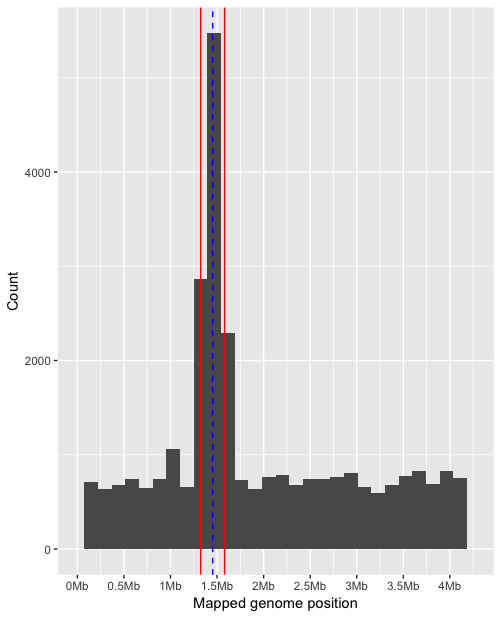
\includegraphics[width=\textwidth]{Chapter_3/Kmer count dupe signal.png}
\caption{Kmers that were more abundant in the genome with the duplication were mapped to the reference genome (X) and a histogram produced. It was clear that there were a high count (Y) of these kmers in the region containing the two copies which is bounded by the red lines. The blue line indicates the junction between the duplicate regions.}
\label{fig:Kmer_abund_is_dece}
\end{figure}

 \begin{figure}[h!]
\centering

\includegraphics[scale=0.6]{universe.jpg}
\caption{Same as above graph but we switch off supplementary alignments.}
\label{fig:Kmer_abund_supp_off}
\end{figure}

\begin{figure}[h!]
\centering
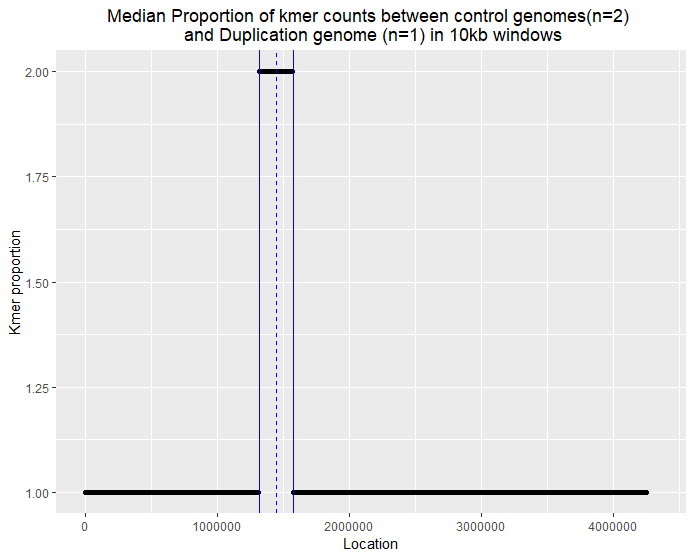
\includegraphics[scale=0.6]{Kmer_dupe.png}
\caption{We can identify the boundry of a dupe using kmers}
\label{fig:kmer_dupe1}
\end{figure}

\end{document}
